\section{Aktueller Stand der Forschung}
\subsection{Allgemeines zur Ausführung einer Kniebeuge}
\noindent Ein sicherer Stand ist die Grundvoraussetzung für eine korrekte Kniebeuge. Beide Füße sollten während der gesamten Bewegung festen Kontakt zum Boden haben, weder die Zehen, noch die Fußkanten oder Fersen dürfen den Boden verlassen. Die optimale Standbreite ist individuell unterschiedlich; Anfänger profitieren häufig von einem etwas breiteren Stand, da dieser zusätzliche Stabilität bietet. Zur Unterstützung können Gegenstände oder ein Trainingspartner zur Stabilisierung herangezogen werden. \cite{Meinart}

\noindent Ein weiterer zentraler Aspekt ist die Haltung des Oberkörpers. Der Rücken bleibt während der gesamten Bewegung gerade, wobei das Becken leicht nach hinten gekippt wird. Insbesondere im Bereich der Lendenwirbelsäule ist eine aktive Rumpfspannung essenziell, um Fehlbelastungen zu vermeiden. \cite{Meinart} Auch biomechanische Analysen zeigen, dass eine neutrale Wirbelsäulenstellung sowie eine kontrollierte Beckenposition entscheidend sind, um Scherkräfte zu minimieren. \cite{schoenfeld2010kinematics}

\noindent Die Kniebeuge folgt stets demselben Bewegungsablauf: Sie beginnt in einer stabilen Ausgangsposition, gefolgt von der exzentrischen Phase (Abwärtsbewegung) und der konzentrischen Phase (Aufwärtsbewegung), bevor erneut die Ausgangsposition eingenommen wird. \cite{Meinart}
\noindent In der folgenden Abbildung 1 ist ein Bewegungsablauf einer Kniebeuge in einzelnen Bewegungsabschnitten abgebildet. Die Abbildung wurde auf Grundlage der Quelle \cite{schoenfeld2010kinematics} und \cite{Meinart} mit KI-gestützter Bildgenerierung (OpenAI DALL·E 3 via ChatGPT, 2025) erstellt. 
\\
\begin{figure}[ht]\centering
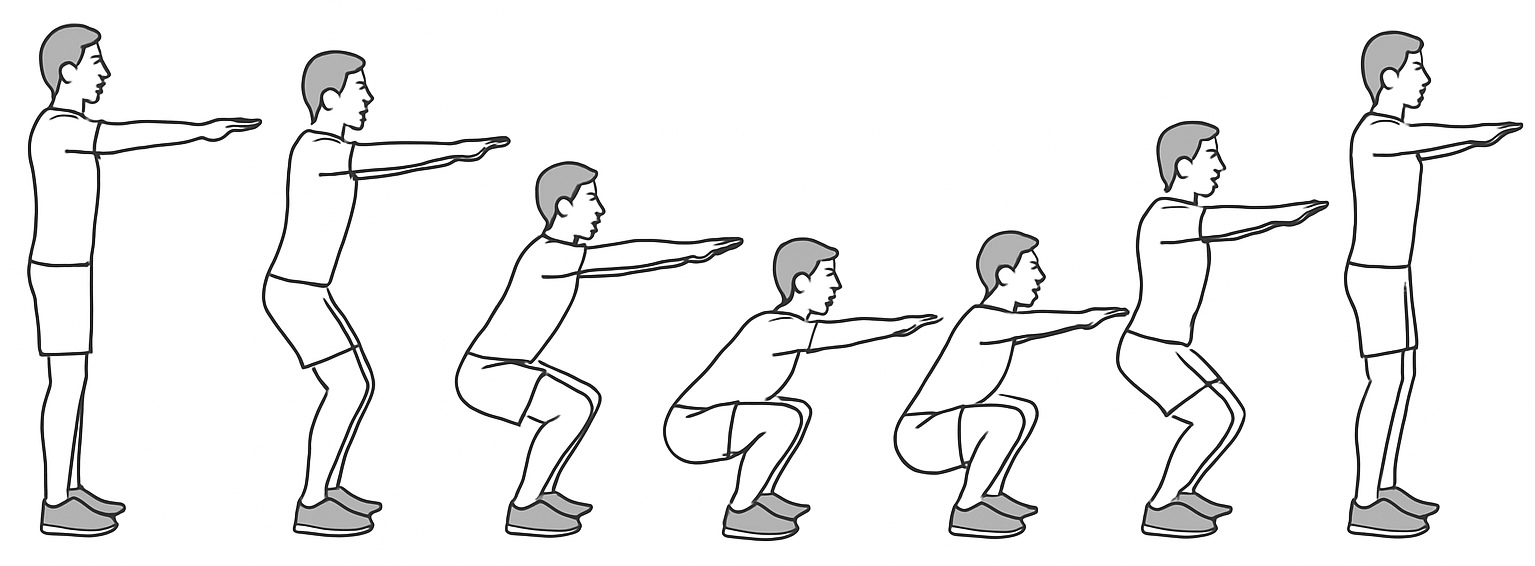
\includegraphics[width=0.75\linewidth]{images/Kniebeuge.jpeg}
\caption{Ablauf einer Kniebeuge, erstellt mit KI-gestützter Bildgenerierung (OpenAI DALL·E 3 via ChatGPT, 2025)}
\label{fig: Kniebeuge}
\end{figure}
\\
\noindent Gestartet wird, wie in Bild 1 zu sehen ist, in aufrechter Haltung. Die Füße stehen schulterbreit und sind leicht nach außen rotiert. Die Arme können zur besseren Balance nach vorne gestreckt werden. Der Rumpf ist angespannt, und die Wirbelsäule befindet sich in einer neutralen Position. \cite{Meinart}

\noindent Wie in Bild 2 dargestellt, wird die Bewegung durch das kontrollierte Zurückschieben des Gesäßes und das Beugen der Knie eingeleitet. Das Körpergewicht bleibt dabei über dem Mittelfuß, während sich der Oberkörper leicht nach vorne neigt. \cite{schoenfeld2010kinematics}

\noindent Während der gesamten Abwärtsbewegung (Bilder 1–3) sollten Hüft-, Knie- und Sprunggelenke gleichzeitig und kontrolliert gebeugt werden. Dabei ist darauf zu achten, dass die Knie nicht über die Fußspitzen hinausragen. \cite{Meinart} Die Kontrolle über die Bewegung wird durch ein bewusst langsames Tempo unterstützt. Studien zeigen, dass eine gute Hüftkontrolle die Belastung auf das Kniegelenk reduziert und die Kraftübertragung optimiert. \cite{schoenfeld2010kinematics} Der Oberkörper sollte möglichst aufrecht bleiben, der Blick nach vorne gerichtet sein, ohne dass der Kopf überstreckt wird. \cite{Meinart}

\noindent Bild 4 zeigt den Tiefpunkt, auch Umkehrpunkt genannt, der Kniebeuge. Je nach Ausführungsvariante ist hier der Kniegelenkswinkel am größten. Die Knie zeigen dabei stabil nach außen. \cite{Meinart}

\noindent Die konzentrische Phase beginnt in Bild 5. Die Aufwärtsbewegung erfolgt durch kraftvolles Drücken aus den Fersen. \cite{schoenfeld2010kinematics} Während der gesamten konzentrischen Phase (Bilder 5–7) sollten Hüft-, Knie- und Sprunggelenke wieder gleichzeitig gestreckt werden. Der Rücken bleibt dabei stabil und gerade, die Füße behalten vollständigen Kontakt zum Boden. \cite{Meinart}

\subsection{Physiologische Grundlagen der Kniebeuge}
\subsubsection{Variationsmöglichkeiten}
\nointent Natürlich gibt es bei der Ausführung einer Kniebeuge verschiedene Variation Möglichkeiten. Zu allem kann eine Kniebeuge mit dem Körpergewicht alleine oder auch mit einem zusätzlichen Gewicht durchgeführt werden. Die Kniebeuge mit der Langhantel ist beispielsweise Bestandteil beim olympischen Gewichtheben. 

\subsubsubsection{Kniebeuge mit Langhantel}
Der grundlegende Bewegungsablauf bei einer Kniebeuge mit Langhantel sollte im Wesentlichen dem einer Körpergewichts Kniebeuge gleichen. Das bedeutet, dass alle Bewegungsmuster, die ohne Zusatzlast bereits sicher beherrscht werden, auch unter Belastung beibehalten werden müssen. Dies ist entscheidend, um Verletzungen vorzubeugen und sicherzustellen, dass durch das zusätzliche Gewicht keine Gelenke oder Muskeln überlastet werden. Besonders wichtig ist dabei eine kontrollierte und stabile Ausführung, bei der die Spannung im gesamten Körper aufrechterhalten wird. \cite{Meinart} Abbildung 2 zeigt drei verschiedene Varianten der Kniebeuge mit einer Langhantel. 
\\
\begin{figure}[ht]\centering
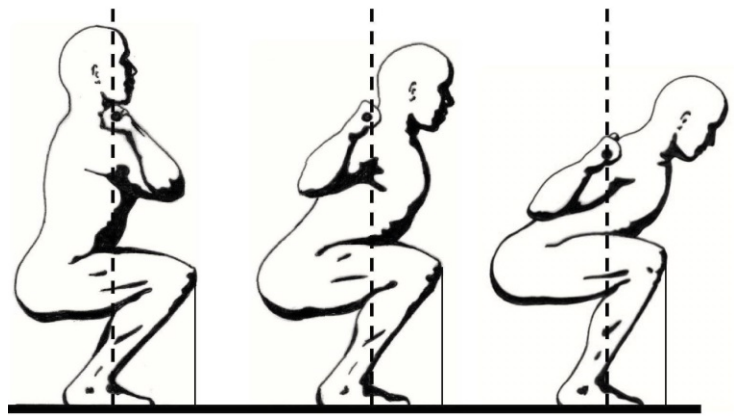
\includegraphics[width=0.75\linewidth]{images/Langhantel_Kniebeuge.png}
\caption{Kniebeugen mit Langhantel, links: Front-Squat, mitte: High Bar, rechts: Low-Bar \cite{Hartmann2014}}
\label{fig: Langhantel}
\end{figure}
\noindent Die Positionierung der Langhantel auf dem Rücken beeinflusst maßgeblich die Körperhaltung während der Kniebeuge. Man unterscheidet hierbei zwischen der „High Bar“- und der „Low Bar“-Technik:
\\
Die „High Bar“-Position ist dadurch gekennzeichnet, dass die Langhantel oberhalb des Schulterdachs auf dem oberen Trapezmuskel abgelegt wird. Diese Variante eignet sich besonders für Anfänger, da sie eine aufrechtere Körperhaltung ermöglicht und den Körperschwerpunkt näher über dem Mittelfuß hält. \cite{Meinart}

\noindent Um die Halswirbelsäule während der Kniebeuge zu schützen, ist es vorteilhaft, eine ausreichende Grundmuskulatur im Nacken- und oberen Rückenbereich aufzubauen. Diese Muskulatur sorgt nicht nur für Stabilität, sondern bietet auch eine natürliche „Polsterung“ für die Langhantel, insbesondere bei der High-Bar-Variante. Ein enger Griff an der Langhantel ist hierbei empfehlenswert. Die Hände sollten so positioniert werden, dass die Unterarme möglichst senkrecht zum Boden stehen. Dies verbessert die Stabilität der Hantel auf dem oberen Rücken und ermöglicht eine präzise Kontrolle während der gesamten Bewegung. \cite{Meinart}
\\
\noindent Im Gegensatz dazu wird die Langhantel beim „Low Bar“-Squat unterhalb des Schulterdach abgelegt. Diese Technik wird häufig bei olympischen Gewichthebern angewendet, da sie eine größere Lastaufnahme ermöglicht. \cite{Meinart}
\noindent Der Griff an der Langhantel kann bei dieser Variante etwas breiter sein, was die Schultergelenke entlastet. Durch die tiefere Ablage der Hantel ergibt sich jedoch eine stärkere Vorlage des Oberkörpers. Diese Vorlage ist notwendig, um den Masseschwerpunkt über dem Mittelfuß zu halten und ein Umfallen nach hinten zu verhindern. durch diese Bewegung Ausführung wird die hintere Muskelkette im Vergleich zur "High Bar" stärker beansprucht. \cite{Meinart}
\\
\noindent Bei der Frontkniebeuge "Front Squat" wird für Fortgeschrittene empfohlen, da diese Ausführung ein höheres Verletzungsrisiko birgt. Die Langhantel wird auf den vorderen Schultern abgelegt, wobei die Hände die Hantel nur stabilisieren und nicht tragen sollen. Der Griff ist leicht breiter als schulterbreit. Die Ellenbogen zeigen nach vorne, die Oberarme bleiben parallel zum Boden, um eine stabile „Front-Rack-Position“ zu gewährleisten. Der Oberkörper sollte möglichst aufrecht bleiben, wobei Gewichtheberschuhe oder erhöhte Fersen dabei unterstützen. Während des gesamten Bewegungsablaufs bleiben Hüfte, Knie und Sprunggelenke synchron in Bewegung, um die Balance zu halten und den Masseschwerpunkt über dem Mittelfuß zu stabilisieren. Alternativ kann die Langhantel in der „Bodybuilding-Variante“ mit überkreuzten Armen gehalten werden, was die Mobilitätsanforderungen reduziert. Die Frontkniebeuge eignet sich ideal zur Kräftigung der vorderen Oberschenkelmuskulatur. \cite{Meinart}

\subsubsection{erreichte Kniegelenkswinkel während einer Kniebeuge}
\noindent Die optimale Tiefe einer Kniebeuge hängt von der individuellen Zielsetzung ab. 
\noindent Für den Muskelaufbau sind tiefe Kniebeugen mit einem Kniewinkel von 40–70° vorteilhaft.\cite{Hartmann2014} Bei korrekter Ausführung und in Abwesenheit von Kniepathologien sind tiefe Kniebeugen nicht schädlich für das Kniegelenk.\cite{Hartmann2014} 

\noindent Bei einer halben Kniebuege spricht man, von einem Kniewinkel von ca. 80-100°. \cite{Hartmann2014} Diese Art der Kniebeuge belastet das Knie häufig mehr als bei einer tiefen Kniebeuge. Dies liegt an den auftretenden Bremskräften kurz vor dem Umkehrpunkt der Bewegung. Im Gegensatz dazu können bei tiefen Kniebeugen die Lasten um 30–50\% geringer sein als bei halben Kniebeugen.\cite{Tiefe}

\noindent Die Viertelkniebeuge entspricht einer geringen Beugung des Knies, im Bereich von ca. 110-140°. \cite{Hartmann2014} In diesem Bereich gibt es wenig Muskelaufbau. Jedoch können hier die größten Lasten gehoben werden. \cite{Tiefe}

\noindent Nach einer Knieverletzung, insbesondere nach einer Kreuzbandverletzung, sollte die Tiefe der Kniebeuge jedoch auf 50–60\% der normalen Bewegung begrenzt werden, um das Gelenk zu entlasten und eine Überlastung der Strukturen zu vermeiden. \cite{Tiefe}

\subsubsection{Allgemein beanspruchte Muskulatur bei einer Kniebeuge}
\noindent Bei einer Kniebeuge sind viele Muskeln beteiligt. Je nach Ausführung variiert die Beanspruchung der Muskulatur. Im folgenden werden die wichtigsten Muskeln in der Kniebeuge aufgelistet. 

\noindent \textbf{Die Wadenmuskulatur} setzt sich aus dem \textbf{M. soleus} und dem \textbf{M. gastrocnemius} zusammen, die während der Kniebeuge unterschiedliche Funktionen erfüllen. Der M. soleus wird vor allem bei einem größeren Kniewinkel aktiviert und spielt in der Aufwärtsbewegung eine zentrale Rolle, da er maßgeblich zur Plantarflexion beiträgt – also zur Bewegung des Fußes im oberen Sprunggelenk in Richtung der Fußsohle. Im Gegensatz dazu unterstützt der M. gastrocnemius sowohl die Plantarflexion als auch die Beugung des Knies, wobei seine Aktivität insbesondere in den ersten 15 Grad der Kniebeuge am höchsten ist. \cite{Meinart}

\noindent \textbf{Der M.gluteus maximus}, der große Gesäßmuskel, ist bei der Kniebeuge sowohl für die Bewegung als auch für die Stabilisierung verantwortlich. Während der Abwärtsbewegung arbeitet er kontrollierend (extentrisch), beim Aufrichten sorgt er für die notwendige Kraftentfaltung (konzentrisch). Er unterstützt die Hüftstreckung und hilft, das Knie zu stabilisieren. Besonders stark beansprucht werden die unteren Muskelanteile, vor allem im tiefsten Punkt der Kniebeuge. \cite{Meinart}

\noindent \textbf{Die ischiocrurale Muskulatur (Hamstring)}, die hintere Oberschenkelmuskulatur, ist während der Kniebeuge nur gering aktiv. Besonders im oberen Bewegungsabschnitt (bei Teilkniebeugen) zeigt sie etwas mehr Aktivität, während die tiefe Kniebeuge kaum zusätzliche Reize setzt. Da der Beinbeuger sowohl für die Beugung des Knies als auch für die Streckung der Hüfte zuständig ist und beide Gelenke während der Kniebeuge gleichzeitig beugen, verändert sich seine Länge kaum. \cite{Meinart}

\noindent \textbf{Der Musculus adductor magnus} ist ein großer, dreieckiger Muskel an der Innenseite des Oberschenkels, der eine wesentliche Rolle bei der Hüftstreckung während der Kniebeuge spielt. Aufgrund seines Ursprungs am Sitzbein (Tuber ischiadicum) wird er oft als “vierter Beinbeuger” bezeichnet, obwohl er nicht am Kniegelenk ansetzt und somit ausschließlich auf die Hüfte wirkt. \cite{Meinart}

\noindent \textbf{Der Musculus quadriceps femoris} besteht aus vier Muskeln. Der Musculus rectus femoris verläuft über Hüft- und Kniegelenk und ermöglicht besonders die Hüftbeugung aber auch Kniestreckung. Der Musculus vastus lateralis, intermedius und medialis liegen am Oberschenkelknochen und sind primär für die Kniestreckung verantwortlich. Für die Kniestabilität ist besonders der Musculus vastos bedeutend. \cite{Meinart}
\\
\noindent In der Abbildung 3 sind die genannten Muskeln und noch weitere Muskeln der Beine abgebildet. 
\\
\begin{figure}[ht]\centering
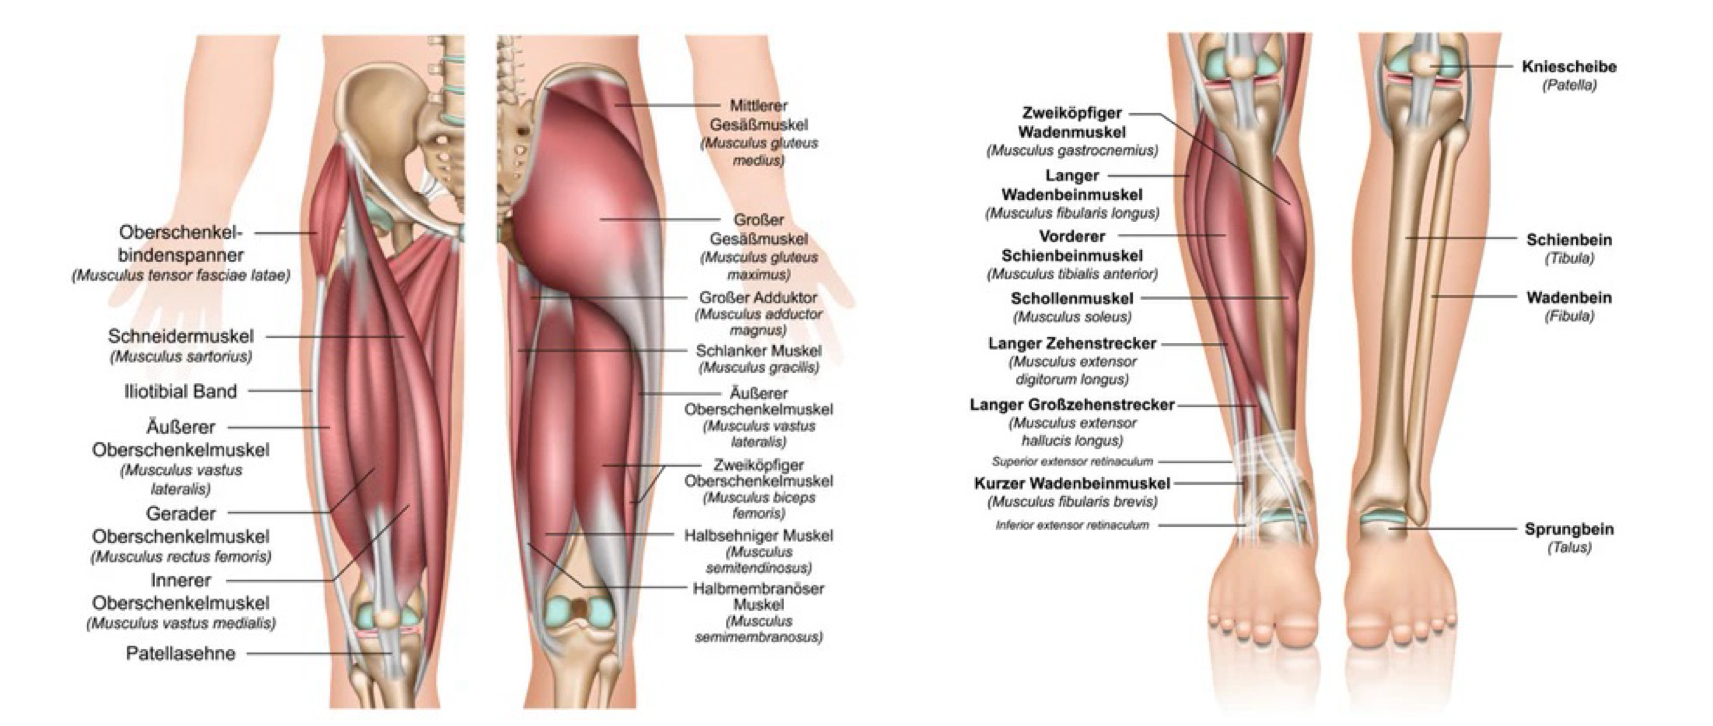
\includegraphics[width=1\linewidth]{images/Muskeln.jpeg}
\caption{Beinmuskulatur (links Oberschenkel, rechts Unterschenkel)\cite{GorillaSports_Beintraining}}
\label{fig: Beinkuskulatur}
\end{figure}
\\
\\
\\
\subsubsection{Vergleich verschiedener Kniebeugen-Tiefen und ihre muskuläre Wirkung}
Die Tiefe einer Kniebeuge hat einen erheblichen Einfluss darauf, welche Muskelgruppen besonders beansprucht werden. Je nach Bewegungsausmaß lassen sich drei wesentliche Varianten unterscheiden: die tiefe Kniebeuge (auch „Ass to Grass“), die halbe Kniebeuge (Parallel Squat) sowie die Viertel-Kniebeuge (Quarter Squat). Jede dieser Varianten aktiviert die Muskulatur in unterschiedlichem Ausmaß.\cite{Meinart}
\\
\\
\noindent \textbf{Die tiefe Kniebeuge} beschreibt eine Ausführung, bei der die Hüfte unterhalb der Kniehöhe absinkt. In dieser Variante werden insbesondere der \textit{Gluteus maximus}, die \textit{Adduktoren} sowie die \textit{Vastus-Gruppe} des Quadrizeps maximal beansprucht. Die große Bewegungsamplitude sorgt für eine starke Dehnung und Aktivierung dieser Muskelgruppen. Vor allem die unteren Fasern des Gluteus maximus sowie der M. adductor magnus arbeiten hier besonders intensiv. Diese Variante ist besonders effektiv für Muskelaufbau, Mobilität und funktionelle Kraft, da sie viele alltagsrelevante Bewegungen abbildet und durch die tiefe Position eine verbesserte Beweglichkeit fördert. \cite{Meinart}
\\
\\
\noindent \textbf{Die halbe Kniebeuge}, bei der die Oberschenkel parallel zum Boden verlaufen, aktiviert primär den Quadrizeps und in geringerem Maße den Gluteus. Die Adduktoren sind in dieser Bewegung nur moderat involviert. Diese Variante ist gelenkschonender als die tiefe Kniebeuge und wird häufig im Kraftdreikampf verwendet, da sie eine gute Balance zwischen Kraftentwicklung und technischer Sicherheit bietet. Durch den reduzierten Bewegungsweg können oft höhere Lasten als bei der tiefen Variante bewegt werden, ohne dabei das Risiko für Überlastung zu erhöhen. \cite{Meinart}
\\
\\
\noindent \textbf{Die Viertel-Kniebeuge} zeichnet sich durch eine sehr geringe Knieflexion aus. Diese Bewegung aktiviert den Beinbeuger (die ischiocrurale Muskulatur) in höherem Maße als die tiefere Variante, da in diesem Bereich die EMG-Aktivität der Hamstrings am stärksten ist. Der Quadrizeps wird hingegen nur minimal beansprucht. Aufgrund der kurzen Bewegungsamplitude eignet sich diese Form insbesondere für Schnellkrafttraining oder sportartspezifische Reize, etwa in Sprungsportarten. Auch im Rehabilitationsbereich kann sie gezielt eingesetzt werden, um Teilbewegungen zu trainieren, ohne die Gelenke zu stark zu belasten. \cite{Meinart}
\\
\\
Zusammenfassend lässt sich sagen, dass die Tiefe der Kniebeuge nicht nur die Belastung der beteiligten Gelenke, sondern vor allem auch die Aktivierung bestimmter Muskelgruppen beeinflusst. Für den gezielten Aufbau von Gesäß- und Adduktorenmuskulatur eignet sich die tiefe Kniebeuge am besten. Wer dagegen den Fokus auf reine Kraftentwicklung oder Schnelligkeit legt, kann von der halben oder gar viertel Kniebeuge profitieren. Die Auswahl der richtigen Variante sollte stets vom Trainingsziel, dem Leistungsstand und der individuellen Anatomie abhängig gemacht werden. \cite{Meinart}

\subsection{Wissenschaftliche Publikation}
\noindent Die präzise Erfassung des Kniegelenkswinkels ist ein zentrales Thema in der orthopädischen Diagnostik, Rehabilitation sowie in sportwissenschaftlichen und medizintechnischen Anwendungen. In den letzten Jahren hat die Forschung erhebliche Fortschritte gemacht. 

\noindent In der Studie „Repeatability of measuring knee flexion angles with wearable inertial sensors“ wurde die Reproduzierbarkeit der Kniewinkelmessung mithilfe tragbarer Inertialsensoren (IMUs) untersucht. Zu diesem Zweck kam ein roboterbetriebenes Beinmodell zum Einsatz, das standardisierte Flexionsbewegungen ausführte, welche Bewegungen wie Kniebeugen simulierten. Zur Erfassung der Bewegungsdaten wurden je ein IMU am Oberschenkel und am Unterschenkel positioniert, jeweils entweder posterior (rückseitig) oder lateral (seitlich). Als Referenzsysteme dienten ein Elektrogoniometer sowie ein optisches 3D-Motion-Capture-System. Die Ergebnisse zeigten, dass beide IMU-Positionierungen eine hohe Wiederholgenauigkeit aufwiesen. Die maximalen Flexionswinkel wurden mit durchschnittlichen Abweichungen von ±1,1° (lateral) bzw. ±2,4° (posterior) im Vergleich zur Referenz gemessen. Während die Bewegungsgeschwindigkeit nur einen geringen Einfluss auf die Messgenauigkeit hatte, führten Positionsveränderungen der Sensoren zu deutlich größeren Messabweichungen. Das lateral angebrachte IMU-Setup erzielte die besten Resultate, was vermutlich auf eine höhere Stabilität und bessere Reproduzierbarkeit der Platzierung zurückzuführen ist. Die Auswertung der Sensordaten erfolgte mittels eines eigens entwickelten MATLAB-Programms zur Berechnung des Kniewinkels. Insgesamt belegt die Studie, dass IMUs in Kombination mit einer softwaregestützten Auswertung eine kosteneffiziente, portable und zugleich zuverlässige Methode zur Messung des Kniewinkels darstellen. Dies gilt insbesondere für dynamische Bewegungsanalysen, wie sie beispielsweise bei Kniebeugen auftreten. Die Autoren schließen daraus, dass IMUs eine valide Alternative zu klassischen Goniometern oder komplexen Motion-Capture-Systemen darstellen. \cite{Fennema2019}
\\
\noindent Ein weiterer Ansatzpunkt ist die Videoanalyse. Sowohl 2D- als auch 3D-basierte Verfahren werden eingesetzt, um Gelenkwinkel nichtinvasiv zu erfassen. Während 3D-Systeme sehr präzise, aber kostenintensiv sind, zeigen aktuelle Studien eine zunehmende Validität auch von 2D-Systemen. 
\\
\noindent In der Studie von Chida et al. (2024) wurde die Validität der zweidimensionalen (2D) Videoanalyse zur Erfassung der Gelenkwinkel der unteren Extremität während eines Fecht-Ausfallschritts untersucht. Ziel war es, die 2D-Analyse als potenziell kostengünstige und praxistaugliche Alternative zur dreidimensionalen (3D) Bewegungsanalyse zu evaluieren. Insgesamt 22 männliche Fechter führten standardisierte Lunge-Bewegungen aus, die gleichzeitig mit einem 3D-Motion-Capture-System (Qualisys) und zwei Digitalkameras aufgezeichnet wurden. Die Analysen konzentrierten sich auf die Zeitpunkte des Abstoßens (heel-off) und des Aufsetzens (heel-strike) des vorderen Beins. Die Ergebnisse zeigten eine sehr hohe Übereinstimmung der Kniewinkel zwischen 2D- und 3D-Analyse bei Abweichungen von maximal ±4,3°, was auf eine hohe Messgenauigkeit der 2D-Methode in der Sagittalebene hinweist. Dagegen zeigten die Messwerte für das Hüft- und Sprunggelenk größere Abweichungen, insbesondere bei der Sprunggelenksanalyse mit einer Überschätzung von bis zu 21,3° durch die 2D-Methode. Die Autoren schlussfolgern, dass die 2D-Videoanalyse eine valide Methode zur Messung des Kniewinkels bei Bewegungen mit geringen Rotationsanteilen darstellen kann. Sie eignet sich besonders für sportpraktische Anwendungen, bei denen keine aufwendige Messtechnik verfügbar ist. \cite{videoanalysis2024}
\nointent Es gibt beispielsweise Anwendungen wie Kniovea, die frei zugänglich sind und zur Winkelanalyse eingesetzt werden. \cite{Kniovea}
